%\documentclass[fontset = none, t, aspectratio=169]{ctexbeamer}
\documentclass[fontset = none, t, aspectratio=169]{ctexbeamer}

% 修改自萧山主题的凤岗主题
\usetheme{nwafufengang}

% 载入需要的宏包
% 加载宏包
%===================注意======================%
% 在调用beamer.cls宏包后,以下宏包将自动调用,
% 不应单独调用这些宏包,以免发生冲突
% amsfonts, amsmath, amssymb, amsthm, 
% enumerate, geometry, graphics, graphicx, 
% hyperref, url, 
% ifpdf, keyval, xcolor, xxcolor
% =============================================%
% % 调整行间距
\usepackage{setspace}

% 生成二维码
\usepackage{qrcode}

% 加载需要的宏包
\usepackage{csquotes}

% 符号字体
\usepackage{fontawesome5}

% unicode数学符号
\usepackage{unicode-math}

\usepackage{multicol}

% ========排版键盘组合和菜单的宏包=========
\usepackage{menukeys}

% ========图像标注宏包=========
%\usepackage{tikz-imagelabels}
\usepackage{tikz-imglabels}
% =========调整项目列表格式=========
%\usepackage{enumitem}

%tikz-imagelabels

%%% Local Variables: 
%%% mode: latex
%%% TeX-master: "../main.tex"
%%% End:


% 进行必要的设置
% 载入字体(需要安装相应字体)
\setmainfont{LibertinusSerif}[% 英文字体
  Extension      = .otf,
  UprightFont    = *-Regular,
  BoldFont       = *-Bold,
  ItalicFont     = *-Italic,
  BoldItalicFont = *-BoldItalic,
  Scale          = 1.0]
%\setmonofont{Iosevka}[Scale=1.0]% 等宽字体,主要用于代码排版
%\setmonofont{Iosevka Term}% 英文等宽字体,主要用于代码排版
\setmathfont{LibertinusMath-Regular.otf}% Iosevka数学字体,需要unicode-math支持
\setCJKmainfont{Source Han Serif SC}[ % 中文衬线字体,思源宋体
  UprightFont     = * SemiBold,
  BoldFont        = * Heavy,
  ItalicFont      = * Light,
  BoldItalicFont  = * Medium,
  RawFeature      = +fwid]
\setCJKsansfont{Source Han Sans SC}[ % 中文无衬线字体,思源宋体
  UprightFont     = * Medium,
  BoldFont        = * Heavy,
  ItalicFont      = * Light,
  BoldItalicFont  = * Normal,
  RawFeature      = +fwid]  
\setCJKmonofont{Sarasa Mono SC}[% 中文等宽字体,Sarasa Mono SC
  UprightFont     = * Medium,
  BoldFont        = * Medium,
  ItalicFont      = * Extralight,
  BoldItalicFont  = * Light,
  RawFeature      = +fwid]   

%% 自定义相关的名称宏命令
%% ==================================================
%% \newcommand{\yourcommand}[参数个数]{内容}
% 西北农林科技大学各单位名称
\newcommand{\nwafu}{西北农林科技大学}
\newcommand{\cie}{信息工程学院}
\newcommand{\ca}{农学院}
\newcommand{\cpp}{植物保护学院}
\newcommand{\ch}{园艺学院}
\newcommand{\cast}{动物科技学院}
\newcommand{\cvm}{动物医学院}
\newcommand{\cf}{林学院}
\newcommand{\claa}{风景园林艺术学院}
\newcommand{\cnre}{资源环境学院}
\newcommand{\cwrae}{水利与建筑工程学院}
\newcommand{\cmee}{机械与电子工程学院}
\newcommand{\cfse}{食品科学与工程学院}
\newcommand{\ce}{葡萄酒学院}
\newcommand{\cls}{生命科学学院}
\newcommand{\cs}{理学院}
\newcommand{\ccp}{化学与药学院}
\newcommand{\cem}{经济管理学院}
\newcommand{\cm}{马克思主义学院}
\newcommand{\dfl}{外语系}
\newcommand{\iec}{创新实验学院}
\newcommand{\ci}{国际学院}
\newcommand{\dpe}{体育部}
\newcommand{\cvae}{成人教育}
\newcommand{\iswc}{水土保持研究所}

%% 签署春秋学期日期命令
\newcommand{\tomonth}{
  \the\year 年\the\month 月
}


\newcommand{\tomonthen}{
  \ifcase\the\month
  \or January%
  \or February%
  \or March%
  \or April%
  \or May%
  \or June%
  \or July%
  \or August%
  \or September%
  \or October%
  \or November%
  \or December%
  \fi, \the\year
}

\newcommand{\tosemester}{
  \the\year 年\ 
  \ifcase\the\month
  \or 秋%
  \or 春%
  \or 春%
  \or 春%
  \or 春%
  \or 春%
  \or 春%
  \or 夏%
  \or 秋%
  \or 秋%
  \or 秋%
  \or 秋%
  \fi 
}

\newcommand{\tosemesteren}{  
  \ifcase\the\month
  \or Autumn%
  \or Spring%
  \or Spring%
  \or Spring%
  \or Spring%
  \or Spring%
  \or Summer%
  \or Autumn%
  \or Autumn%
  \or Autumn%
  \or Autumn%
  \or Autumn%
  \fi, \the\year
}

% 插图路径设置
% ==================================================
\graphicspath{{figs/}}%图片所在的目录
% ==================================================

%改变脚注的符号
\setbeamerfont{footnote}{size=\zihao{7}} % 改变脚注字号
\makeatletter
\def\@fnsymbol#1{\ensuremath{\ifcase#1\or *\or \dagger\or \ddagger\or
   \mathsection\or \mathparagraph\or \|\or **\or \dagger\dagger
   \or \ddagger\ddagger \else\@ctrerr\fi}}
\makeatother
\renewcommand{\thefootnote}{\fnsymbol{footnote}}

\DeclareRobustCommand{\nonumberfootnote}[2][]{%
  \let\thefootnote\relax
  \footnotetext#1{#2}}    

\makeatletter
\def\@fnsymbol#1{\ensuremath{\ifcase#1\or *\or \dagger\or \ddagger\or
   \mathsection\or \mathparagraph\or \|\or **\or \dagger\dagger
   \or \ddagger\ddagger \else\@ctrerr\fi}}
\renewcommand{\thefootnote}{\fnsymbol{footnote}}
\makeatother

% PoZheHao, see https://github.com/CTeX-org/ctex-kit/issues/382
\ExplSyntaxOn
\xeCJK_new_class:n { PoZheHao }
\__xeCJK_save_CJK_class:n { PoZheHao }
\xeCJK_declare_char_class:nn { PoZheHao } { "2014 }
\seq_map_inline:Nn \g__xeCJK_class_seq
  {
    \str_if_eq:nnF {#1} { PoZheHao }
      {
        \xeCJK_copy_inter_class_toks:nnnn { PoZheHao } {#1} { FullRight } {#1}
        \xeCJK_copy_inter_class_toks:nnnn {#1} { PoZheHao } {#1} { FullRight }
      }
  }
\ExplSyntaxOff

% 超链接及符号
\newcommand\link[1]{\href{#1}{\ \faExternalLinkSquare*}}  

% TikZ宏包扩展
\usetikzlibrary{fit}
% \usetikzlibrary{graphs}
% \usetikzlibrary{mindmap,trees}
%Here we change the style for all concepts: (Stefan K.)
% \tikzset{every concept/.style={minimum size=1cm, text width=1.5cm}}
% \usetikzlibrary{shapes,arrows,chains}
% \usetikzlibrary{positioning}
% \usetikzlibrary{calc}
% \usetikzlibrary{arrows.meta}
% \usetikzlibrary{decorations.pathreplacing}
% \usetikzlibrary{tikzmark}
% \usetikzlibrary{shapes.geometric}
% \usetikzlibrary{decorations.text}
% \usetikzlibrary{matrix}
% \usetikzlibrary{backgrounds}

% 设置minted宏包编排代码的参数及用于latex代码排版的简化命令
\setminted{fontsize=\footnotesize, breaklines=true, breakautoindent=false}
\newmintinline{tex}{fontsize=\footnotesize}
\newmintinline{sh}{breaklines=true}
\newmintinline[texinlinett]{tex}{escapeinside=||}
\newminted{tex}{fontsize=\scriptsize, bgcolor=yellow!20, frame=lines, autogobble}
\newminted[texcodett]{tex}{autogobble, fontsize=\scriptsize, bgcolor=yellow!20, frame=lines, escapeinside=||}
\newminted[shell]{sh}{autogobble,frame=lines}
\newmintedfile{tex}{bgcolor=yellow!20, fontsize=\footnotesize, frame=lines}

%====================用tcolorbox定义一个代码盒子==============================
\tcbuselibrary{skins, xparse, minted}
%\usetikzlibrary{shapes.geometric}
%------------------------------------------------------------------------------------
% tcolorbox lang代码样式定义
%------------------------------------------------------------------------------------
\tcbset{%
  lang/.style={%
    drop shadow,%    
    arc=0mm,%
    right=0pt,%
    top=0pt,%
    bottom=0pt,%
    left=0pt,%
    enhanced jigsaw,
    %text width = \textwidth,
    %righthand width=3cm,
    %lowerbox=invisible,
    %lower separated=false,        
    %colframe=tcbcolback!60!black,%
    colframe=blue!50!black,%
    colback=yellow!20,%tcbcolback!30!white,%
    colbacktitle=tcbcolback!5!yellow!10!white,%
    fonttitle=\scriptsize\bfseries,%
    coltitle=black,%
    attach boxed title to top left={%
      xshift=0.6cm,%
      yshift*=0.5mm-\tcboxedtitleheight%
    },%
    %varwidth boxed title*=-3cm,%
    boxed title style={%
      frame code={%
        \path[fill=blue!55!black]([yshift=-1mm,xshift=-1mm]frame.north west)%
        arc[start angle=0,end angle=180,radius=1mm]([yshift=-1mm,xshift=1mm]frame.north east)%
        arc[start angle=180,end angle=0,radius=1mm];%
        \path[left color=tcbcolback!60!black,right color=tcbcolback!60!black,
        middle color=tcbcolback!80!black]([xshift=-2mm]frame.north west)%
        --([xshift=2mm]frame.north east)[rounded corners=1.0mm]%
        --([xshift=1mm,yshift=-1mm]frame.north east)%
        --(frame.south east)%
        --(frame.south west)%
        --([xshift=-1mm,yshift=-1mm]frame.north west)[sharp corners]%
        --cycle;%
      },%
      interior engine=empty,% 
      size=small,
      top=-1mm,
      bottom=-1mm,
    },%
  }% 
}% end tcolorbox lang style

% ===================================
% langPyOne environment definition 
% ===================================
\DeclareTCBListing{texcb}{ O{} m }{%
  listing engine=minted,%
  minted style=default,%
  minted options={%
    breaklines,%
    fontsize=\scriptsize,%
    %linenos,%
    %numbersep=1mm%
    escapeinside=#1,
    autogobble,
  },%
  listing only,%
  lang,%
  title={#2},%
  minted language=tex%
}% end codebox
% ===========================================================


%%% Local Variables: 
%%% mode: latex
%%% TeX-master: "../main.tex"
%%% End: 


% Information
\title[pdfReview]{\Large PDF文件常用修订软件及操作}

%\subtitle{凤岗主题 V\ 2.0}

\author[N. Geng]{耿楠}

\date{\tosemester} % 也可以使用类似\date[2017/04/20]{\zhdate{2017/04/20}}的
              % 方式指定时间

\institute[教发中心]{教学发展中心\\西北农林科技大学}

\titlegraphic{%
  \vspace{3.0cm}
  \qrcode[hyperlink, height=1.6cm]{https://github.com/registor/pdfReview}}

\begin{document}

\begin{frame}[plain,noframenumbering]
  \maketitle
\end{frame}

%\tableofcontents

\begin{frame}{目录}{主要内容}
  %\centering
  \begin{multicols}{2}
    %\centering
    \tableofcontents
  \end{multicols}  
\end{frame}

\section{PC计算机}
\subsection{Acrobat Reader}
\begin{frame}{PC计算机}{Acrobat Reader DC}
  \begin{columns}[c]
    \column{0.35\textwidth}
    \begin{itemize}
    \item 基本功能
      \begin{itemize}
      \item 查看、打印PDF文档
      \item \alert{注释}PDF文档
      \item 表单和多媒体交互
      \end{itemize}
    \item 适用平台
      \begin{itemize}
      \item Windows
      \item Mac OS
      \item Android
      \end{itemize}
    \item 下载链接
      \begin{itemize}
      \item 官网\link{https://get.adobe.com/cn/reader/otherversions/}
      \end{itemize}
    \item 授权
      \begin{itemize}
      \item \alert{免费}
      \end{itemize}
    \end{itemize}
    \column{0.55\textwidth}
    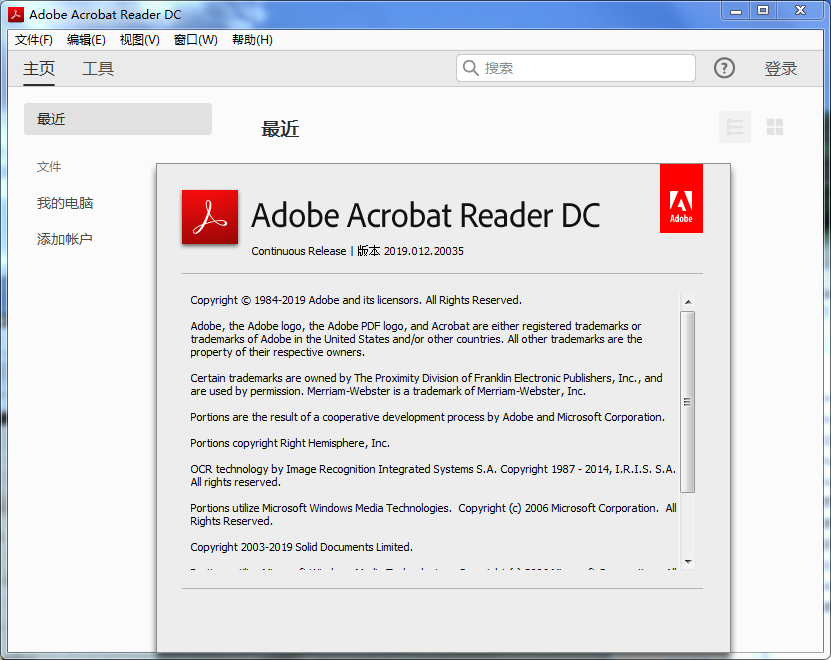
\includegraphics[width=0.9\textwidth]{01acrobat/01aboutacrobatreaderdc}
  \end{columns}
\end{frame}

\begin{frame}{PC计算机}{Acrobat Reader DC}
  \begin{columns}[T]
    \column{0.55\textwidth}
    \begin{itemize}
    \item 打开\enquote{注释}工具栏
      \begin{itemize}\itemsep=5pt%[itemsep=10pt]
      \item \menu{视图>工具>注释>打开}
      \item 工具边栏\keys{注释}图标
      \end{itemize}
    \end{itemize}
    \begin{center}
      \begin{annotationimage}{width=0.9\textwidth}{01acrobat/02openreviewtools01}
        % 利用fit库绘制命名矩形
        \node[fit={(0.145,0.89) (0.235,0.96)}, inner sep=0pt, draw=red, thick] (view) {};
        \node[fit={(0.23,0.53) ($(0.23, 0.53) + (0.07, 0.045)$)}, inner sep=0pt, draw=red, thick] (tools) {};
        \node[fit={(0.522,0.52) ($(0.522, 0.52) + (0.05, 0.045)$)}, inner sep=0pt, draw=red, thick] (annotation) {};
        \node[fit={(0.755,0.52) ($(0.755, 0.52) + (0.075, 0.045)$)}, inner sep=0pt, draw=red, thick] (open) {};
        % 绘制箭头连线表示操作顺序
        \draw[-{Stealth[scale=0.8]}, blue, thick] (view.south) to [out=-90, in=180] (tools.west);
        \draw[-{Stealth[scale=0.8]}, blue, thick] (tools.east) to [out=0, in=180] (annotation.west);
        \draw[-{Stealth[scale=0.8]}, blue, thick] (annotation.east) to [out=0, in=180] (open.west);
      \end{annotationimage}
    \end{center}    
    \column{0.45\textwidth}
    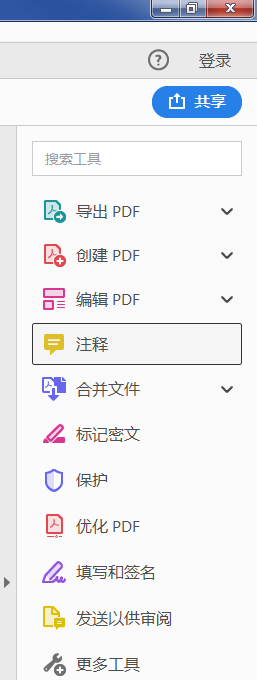
\includegraphics[height=0.8\textheight]{01acrobat/03openreviewtools02}\qquad
    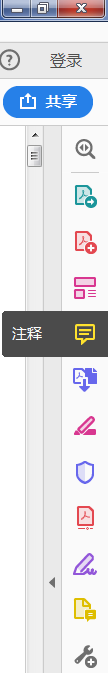
\includegraphics[height=0.8\textheight]{01acrobat/03openreviewtools03}
  \end{columns}
\end{frame}

\begin{frame}{PC计算机}{Acrobat Reader DC}
  \begin{itemize}
  \item \enquote{注释}工具栏
    \begin{itemize}
    \item 用于添加各类注释
    \end{itemize}
  \end{itemize}
  \begin{center}
    \begin{annotationimage}{width=0.8\textwidth}{01acrobat/03openreviewtools04}
        % 利用fit库绘制命名矩形
        \node[fit={(0.285,0.81) (0.72, 0.85)}, inner sep=0pt, draw=red, thick] (tools) {};
        % 绘制说明标记
        \node (annotation) [red,right=of tools,shift={(-0.06, -0.15)}] {\small \enquote{注释}工具栏};
        % 绘制箭头连线表示操作顺序
        \draw[-{Stealth[scale=0.8]}, blue, thick] (annotation.north) to [out=90, in=0] (tools.east);
      \end{annotationimage}
  \end{center}
\end{frame}

\begin{frame}{PC计算机}{Acrobat Reader DC}
  \begin{itemize}
  \item \enquote{注释}工具栏
    \begin{itemize}
    \item \enquote{批注}工具
    \end{itemize}
  \end{itemize}
  
  \begin{center}
    \begin{annotationimage}{width=0.8\textwidth}{01acrobat/03reviewicons01}
      % 绘制外观设置按钮分组示意下划线
      \draw[thick,blue] (0.86,0.26) -- (1.0,0.26);
      % 添加各图标标注
      \foreach \ann/\xpos in
      {
        {附\\注\\工\\具}/0.02, {高\\亮\\工\\具}/0.07,
        {下\\划\\线\\工\\具}/0.126, {删\\除\\线\\工\\具}/0.18,
        {删\\除\\线\\并\\插\\入\\附\\注\\工\\具}/0.229, {插\\入\\文\\本\\工\\具}/0.283,
        {文\\本\\工\\具}/0.346, {文\\本\\框\\工\\具}/0.40,
        {铅\\笔\\绘\\图\\工\\具}/0.45, {铅\\笔\\擦\\工\\具}/0.51,
        {图\\章\\工\\具}/0.56, {附\\加\\文\\件\\工\\具}/0.63,
        {绘\\图\\工\\具}/0.7, {保\\持\\选\\择\\工\\具}/0.79,
        {注\\释\\外\\观\\设\\置}/0.93
      }
      {
        \draw[annotation below = {{\ann} at \xpos}] to (\xpos,0.48);
      }
      % \draw[annotation below = {附\\注\\工\\具 at 0.02}] to (0.02,0.5);
      % \draw[annotation below = {高\\亮\\工\\具 at 0.07}] to (0.07,0.5);
      % \draw[annotation below = {下\\划\\线\\工\\具 at 0.126}] to (0.126,0.5);
      % \draw[annotation below = {删\\除\\线\\工\\具 at 0.18}] to (0.18,0.5);
      % \draw[annotation below = {删\\除\\附\\注\\工\\具 at 0.229}] to (0.229,0.5);
      % \draw[annotation below = {插\\入\\文\\本\\工\\具 at 0.283}] to (0.283,0.5);
      % \draw[annotation below = {文\\本\\工\\具 at 0.346}] to (0.346,0.5);
      % \draw[annotation below = {文\\本\\框\\工\\具 at 0.40}] to (0.40,0.5);
      % \draw[annotation below = {铅\\笔\\绘\\图\\工\\具 at 0.45}] to (0.45,0.5);
      % \draw[annotation below = {铅\\笔\\擦\\工\\具 at 0.51}] to (0.51,0.5);
      % \draw[annotation below = {图\\章\\工\\具 at 0.56}] to (0.56,0.5);
      % \draw[annotation below = {附\\加\\文\\件\\工\\具 at 0.63}] to (0.63,0.5);
      % \draw[annotation below = {绘\\图\\工\\具 at 0.7}] to (0.7,0.5);
      % \draw[annotation below = {保\\持\\选\\择\\工\\具 at 0.79}] to (0.79,0.5);
      % \draw[thick,blue] (0.86,0.28) -- (1.0,0.28);
      % \draw[annotation below = {注\\释\\外\\观\\设\\置 at 0.93}] to (0.93,0.5); 
      % 附注工具、高亮工具、下划线工具、删除线工具、删除附注工具、插入
      % 文本工具、文本注释工具、文本框工具、铅笔工具、铅笔橡皮擦工具、图章工具、附
      % 加文件、绘图工具、保持选择工具、注释的外观工具
    \end{annotationimage}
  \end{center}
\end{frame}

\begin{frame}{PC计算机}{Acrobat Reader DC}
  \begin{itemize}
  \item 使用\enquote{批注}工具添加注释
    \begin{itemize}
    \item 详见:\link{https://helpx.adobe.com/cn/acrobat/using/commenting-pdfs.html}
    \end{itemize}
  \end{itemize}
  
  \begin{center}
    \begin{annotationimage}{width=0.55\textwidth}{01acrobat/04adddeleteline}      
    \end{annotationimage}
    \begin{annotationimage}{width=0.55\textwidth}{01acrobat/04addtextbox}      
    \end{annotationimage}
  \end{center}
\end{frame}

\begin{frame}{PC计算机}{Acrobat Reader DC}
  \begin{columns}[t]
    \column{0.35\textwidth}
    \begin{itemize}
    \item 管理注释
      \begin{itemize}\itemsep=10pt
      \item 复制
      \item 编辑
      \item 删除
      \item 设置状态
      \item 属性
      \item 添加勾形
      \end{itemize}
    \end{itemize}
    \column{0.45\textwidth}
    \begin{center}
      \begin{annotationimage}{height=0.75\textheight}{01acrobat/04editreviewcontents}
      \end{annotationimage}
    \end{center}
  \end{columns}
\end{frame}

\subsection{Foxit福昕}
\begin{frame}{PC计算机}{Foxit福昕}
  \begin{columns}[c]
    \column{0.35\textwidth}
    \begin{itemize}
    \item 基本功能
      \begin{itemize}
      \item 查看、打印PDF文档
      \item \alert{注释}PDF文档
      \item 其它
      \end{itemize}
    \item 适用平台
      \begin{itemize}
      \item Windows
      \item Mac OS
      \item Linux
      \item Android
      \item iOS
      \end{itemize}
    \item 下载链接
      \begin{itemize}
      \item 官网\link{https://www.foxitsoftware.cn/downloads/}
      \end{itemize}
    \item 授权
      \begin{itemize}
      \item \alert{免费}
      \end{itemize}
    \end{itemize}
    \column{0.55\textwidth}
    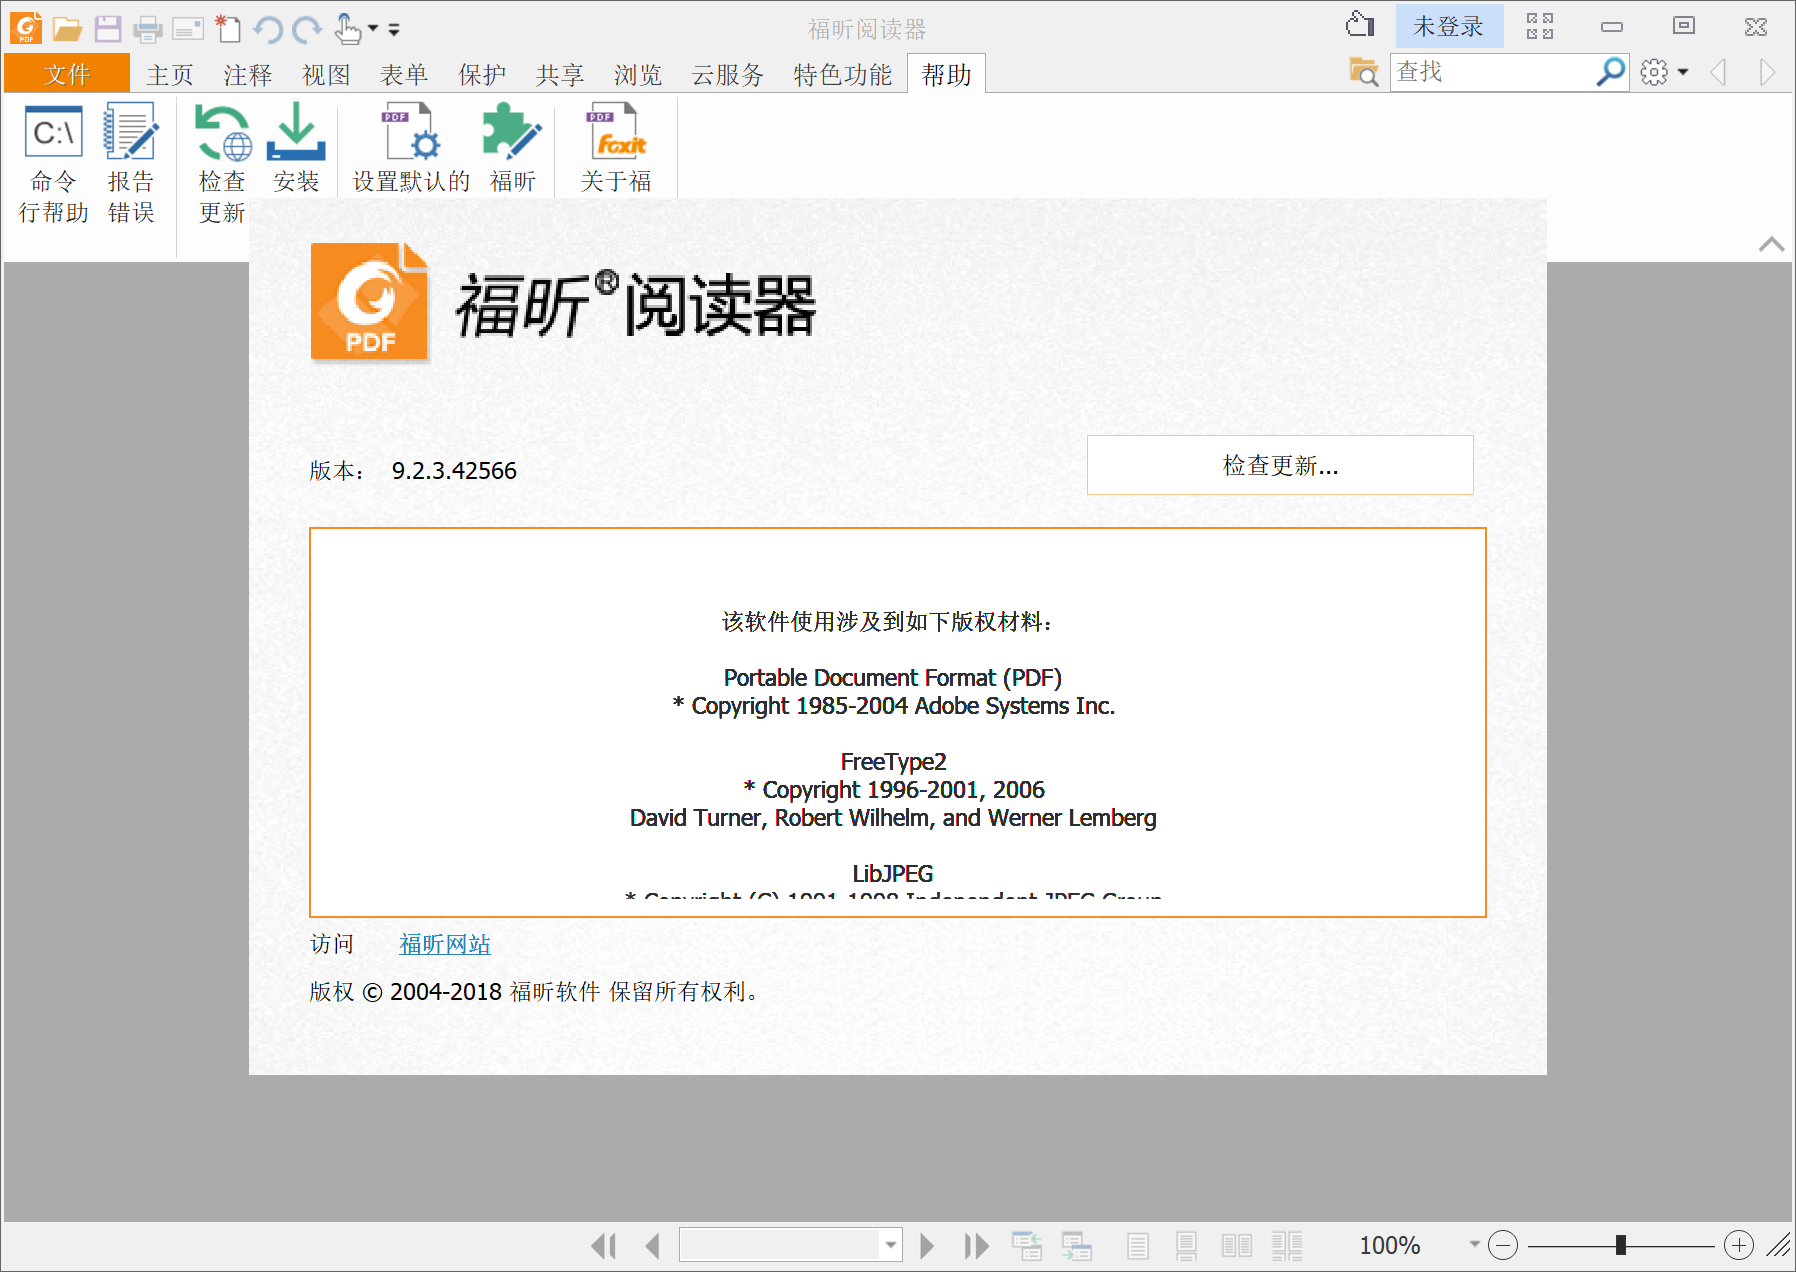
\includegraphics[width=1.0\textwidth]{02foxitreader/01foxitabout}
  \end{columns}
\end{frame}

\begin{frame}{PC计算机}{Foxit福昕}
  \begin{itemize}
  \item \enquote{注释}工具栏
    \begin{itemize}
    \item \menu{注释}菜单打开\enquote{注释}工具栏
    \end{itemize}
  \end{itemize}
  \begin{center}
    \begin{annotationimage}{width=0.9\textwidth}{02foxitreader/03foxitanntoolbar}
    \end{annotationimage}
  \end{center}
\end{frame}

\begin{frame}{PC计算机}{Foxit福昕}
  \begin{itemize}
  \item \enquote{注释}工具栏
    \begin{itemize}
    \item 添加各类\enquote{注释}\footnote[frame,1]{与Acrobat Reader DC
        软件操作基本一致。}
    \item 管理各类\enquote{注释}
    \end{itemize}
  \end{itemize}
  \begin{center}
    \begin{annotationimage}{width=0.5\textwidth}{02foxitreader/02foxitgui}
    \end{annotationimage}
  \end{center}
\end{frame}


\subsection{金山PDF}
\begin{frame}{PC计算机}{金山PDF}
  \begin{columns}[c]
    \column{0.35\textwidth}
    \begin{itemize}
    \item 基本功能
      \begin{itemize}
      \item 查看、打印PDF文档
      \item \alert{注释}PDF文档
      \item 其它
      \end{itemize}
    \item 适用平台
      \begin{itemize}
      \item Windows
      \item 其它平台未知
      \end{itemize}
    \item 下载链接
      \begin{itemize}
      \item 官网\link{https://www.wps.cn/product/kingsoftpdf/}
      \end{itemize}
    \item 授权
      \begin{itemize}
      \item \alert{免费}
      \end{itemize}
    \end{itemize}
    \column{0.55\textwidth}
    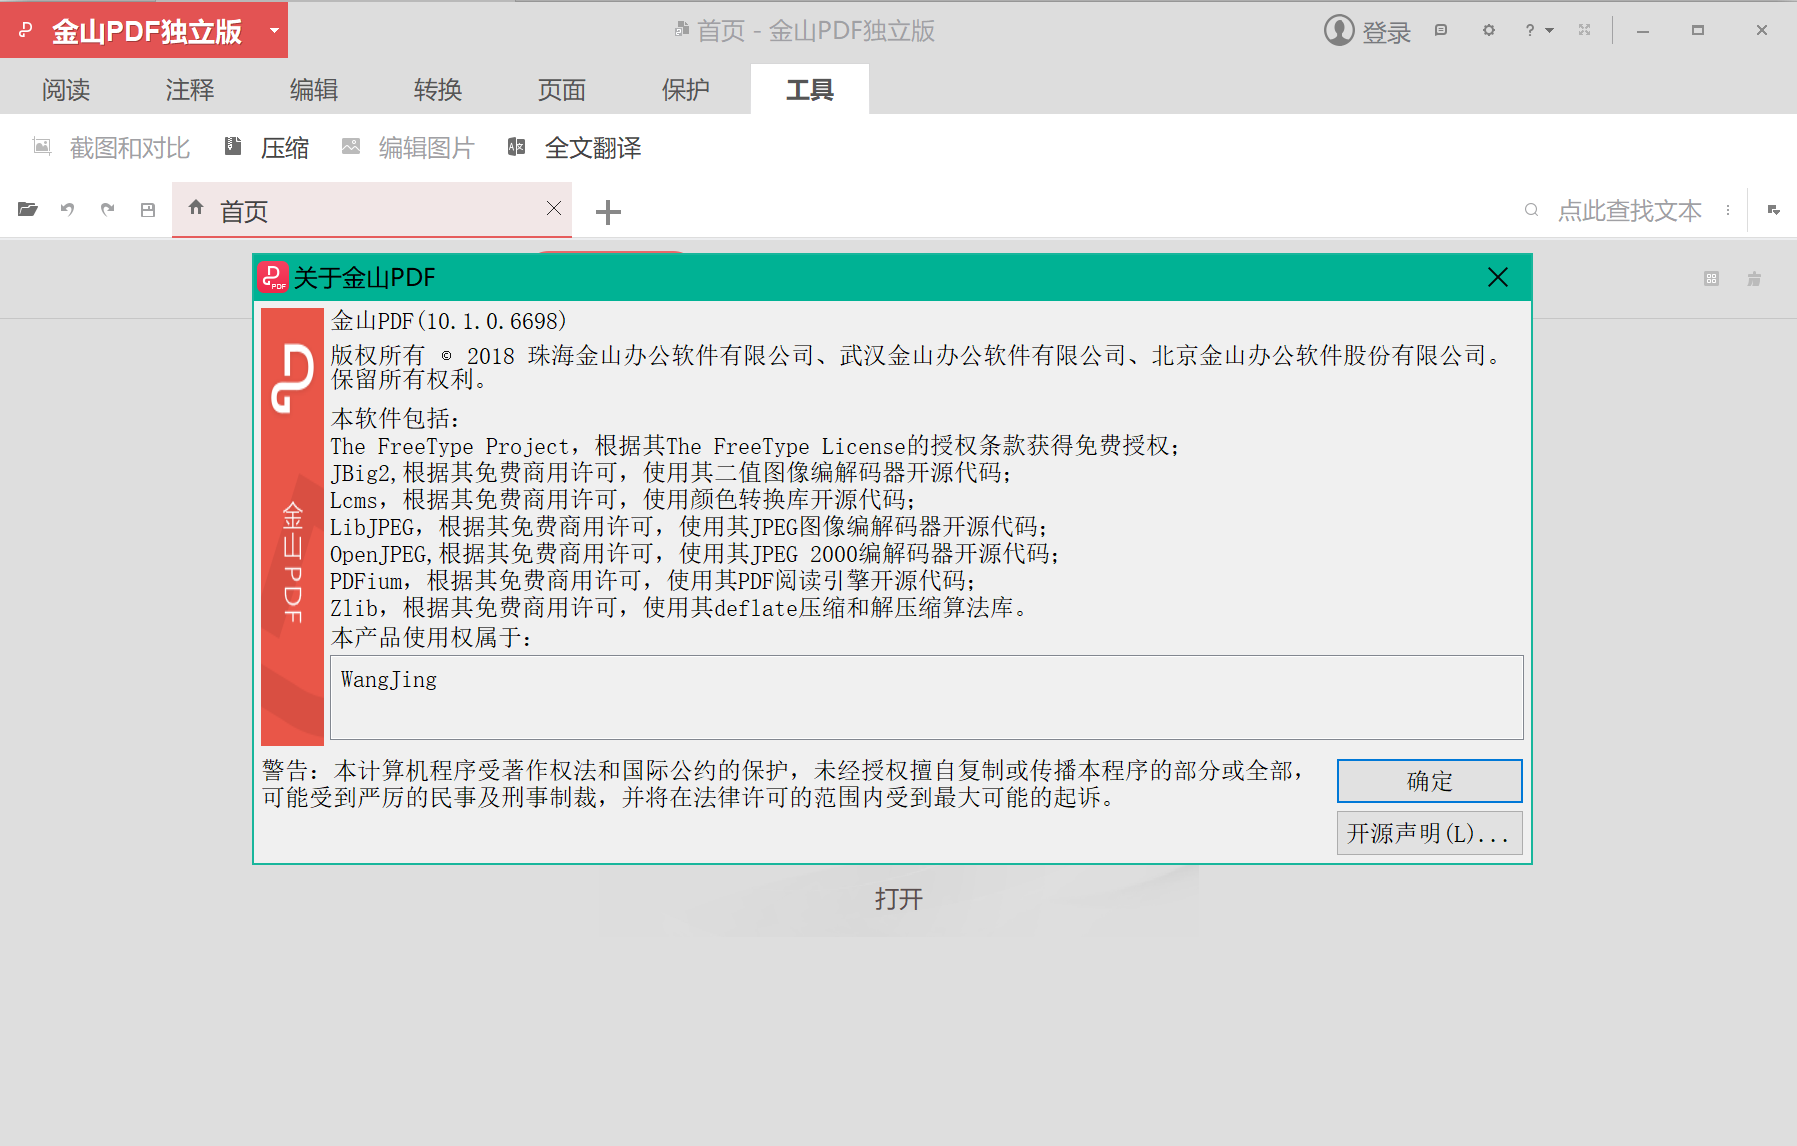
\includegraphics[width=1.0\textwidth]{03kingsoftpdf/01kingsoftpdfabout}
  \end{columns}
\end{frame}

\begin{frame}{PC计算机}{金山PDF}
  \begin{itemize}
  \item \enquote{注释}工具栏
    \begin{itemize}
    \item \menu{注释}菜单打开\enquote{注释}工具栏
    \end{itemize}
  \end{itemize}
  \begin{center}
    \begin{annotationimage}{width=0.9\textwidth}{03kingsoftpdf/03kingsoftpdfanntoolbar}
    \end{annotationimage}
  \end{center}
\end{frame}

\begin{frame}{PC计算机}{金山PDF}
  \begin{itemize}
  \item \enquote{注释}工具栏
    \begin{itemize}
    \item 添加各类\enquote{注释}\footnote[frame,1]{与Acrobat Reader DC
        软件操作基本一致。}
    \item 管理各类\enquote{注释}\footnote[frame,2]{注意使用
        \enquote{\alert{超级注释模式}}。}
    \end{itemize}
  \end{itemize}
  \begin{center}
    \begin{annotationimage}{width=0.5\textwidth}{03kingsoftpdf/042kingsoftpdfsuper}
    \end{annotationimage}
  \end{center}
\end{frame}

\subsection{Okular}
\begin{frame}{PC计算机}{Okular}
  \begin{columns}[c]
    \column{0.35\textwidth}
    \begin{itemize}
    \item 基本功能
      \begin{itemize}
      \item 查看、打印PDF文档
      \item \alert{注释}PDF文档
      \item 其它
      \end{itemize}
    \item 适用平台
      \begin{itemize}
      \item Windows
      \item Mac OS
      \item Linux
      \end{itemize}
    \item 下载链接
      \begin{itemize}
      \item 官网
        \link{https://okular.kde.org/}\footnote[frame,1]{Ubuntu平台可
          以直接使用:sudo apt install okular命令进行安装。}
      \end{itemize}
    \item 授权
      \begin{itemize}
      \item \alert{免费}
      \end{itemize}
    \end{itemize}
    \column{0.55\textwidth}
    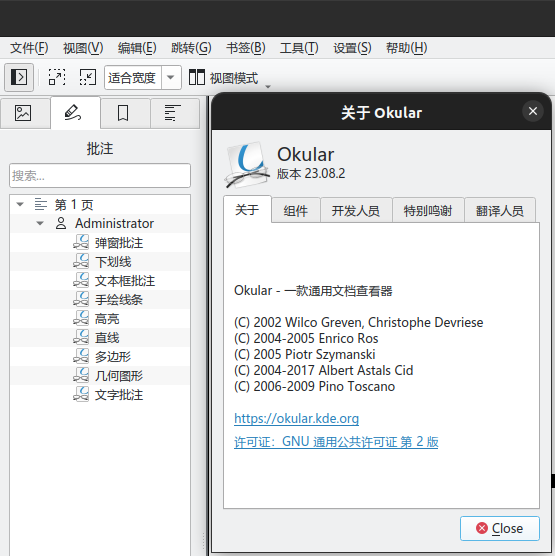
\includegraphics[width=0.95\textwidth]{04okular/01okularabout}
  \end{columns}
\end{frame}

\begin{frame}{PC计算机}{Foxit福昕}
  \begin{itemize}
  \item \enquote{注释}工具栏
    \begin{itemize}
    \item \menu{注释}菜单打开\enquote{注释}工具栏
    \end{itemize}
  \end{itemize}
  \begin{center}
    \begin{annotationimage}{height=0.7\textheight}{04okular/03okulartoolbar}
    \end{annotationimage}
  \end{center}
\end{frame}

\begin{frame}{PC计算机}{Foxit福昕}
  \begin{itemize}
  \item \enquote{注释}工具栏
    \begin{itemize}
    \item 添加各类\enquote{注释}\footnote[frame,1]{与Acrobat Reader DC
        软件操作基本一致。}
    \item 管理各类\enquote{注释}
    \end{itemize}
  \end{itemize}
  \begin{center}
    \begin{annotationimage}{width=0.6\textwidth}{04okular/02okulargui}
    \end{annotationimage}
  \end{center}
\end{frame}
\begin{frame}[standout,plain]
  说明:\\
  软件其他功能也很强大\\
  只要\alert{熟悉一个软件}就好\\
  \alert{推荐}使用\enquote{Acrobat Reader DC},毕竟是\alert{原生的}\\
  肯定还有你偏好的其它软件
  % \begin{itemize}\itemsep=5pt
  % \item 软件其他功能也很强大
  % \item 只要\alert{熟悉一个软件}就好
  % \item 推荐使用\enquote{Acrobat Reader DC},毕竟是\alert{原生的}。
  % \item 肯定还有你偏好的其它软件 
  % \end{itemize}
\end{frame}
\section{iOS平板}
\subsection{Goodnotes}
\begin{frame}{iOS平板}{Goodnotes}
  \begin{columns}[c]
    \column{0.45\textwidth}
    \begin{itemize}\itemsep=3pt
    \item 基本功能
      \begin{itemize}
      \item 笔记软件
      \item 支持Apple Pencil
      \item 可以\alert{批注}PDF文档
      \item 具备文字识别功能(OCR)
      \end{itemize}
    \item 适用平台
      \begin{itemize}
      \item iOS平板
      \item 其它平台未知
      \end{itemize}
    \item 下载链接
      \begin{itemize}
      \item Apple Store
      \end{itemize}
    \item 授权
      \begin{itemize}
      \item \alert{50.00RMB}
      \end{itemize}
    \end{itemize}
    \column{0.45\textwidth}
    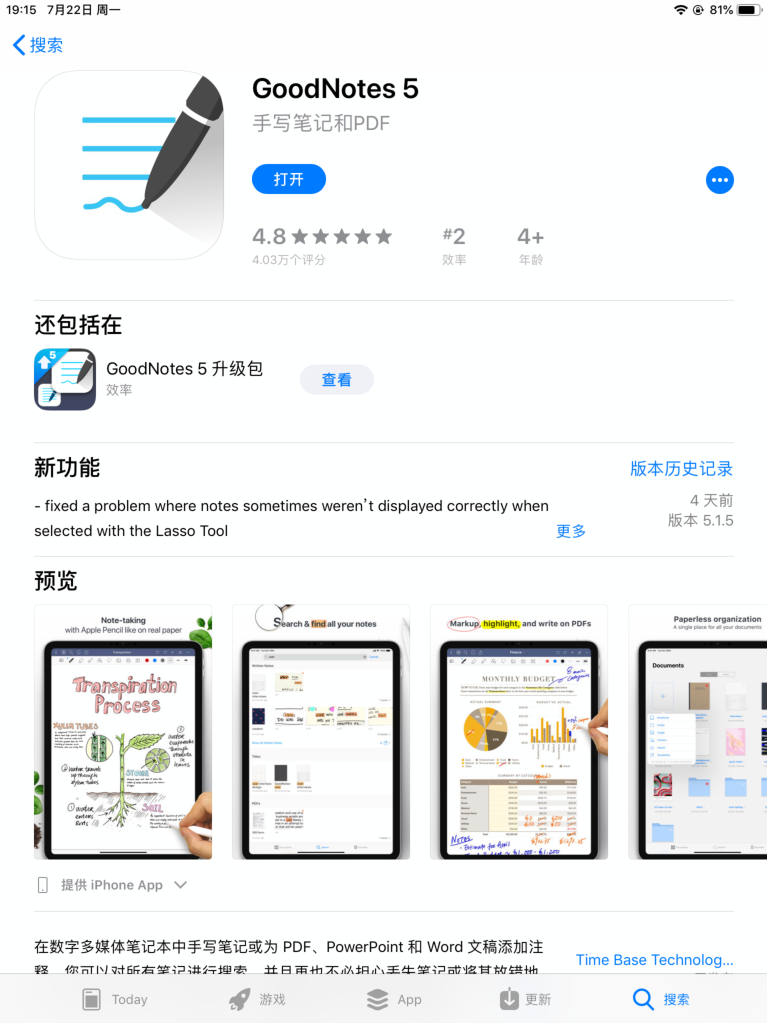
\includegraphics[height=0.75\textheight]{05goodnotes/01goodnotesappstore}
  \end{columns}
\end{frame}

\subsection{Notability}
\begin{frame}{iOS平板}{Notability}
  \begin{columns}[c]
    \column{0.45\textwidth}
    \begin{itemize}\itemsep=3pt
    \item 基本功能
      \begin{itemize}
      \item 笔记软件
      \item 支持Apple Pencil
      \item 可以\alert{批注}PDF文档
      \end{itemize}
    \item 适用平台
      \begin{itemize}
      \item iOS平板
      \item 其它平台未知
      \end{itemize}
    \item 下载链接
      \begin{itemize}
      \item Apple Store
      \end{itemize}
    \item 授权
      \begin{itemize}
      \item \alert{68.00RMB}
      \end{itemize}
    \end{itemize}
    \column{0.45\textwidth}
    
\includegraphics[height=0.75\textheight]{06notability/01notabilityappstore}
  \end{columns}
\end{frame}

\section{\LaTeX 源码修订}
\subsection{changes宏包}
\subsection{todonotes宏包}
\subsection{pdfreview宏包}

%\section{小结}
\begin{frame}[standout,plain]
  ...
\end{frame}

\end{document}

%%% Local Variables:
%%% mode: latex
%%% TeX-master: t
%%% End:
